\documentclass[ignorenonframetext,]{beamer}
\setbeamertemplate{caption}[numbered]
\setbeamertemplate{caption label separator}{: }
\setbeamercolor{caption name}{fg=normal text.fg}
\beamertemplatenavigationsymbolsempty
\usepackage{lmodern}
\usepackage{amssymb,amsmath}
\usepackage{ifxetex,ifluatex}
\usepackage{fixltx2e} % provides \textsubscript
\ifnum 0\ifxetex 1\fi\ifluatex 1\fi=0 % if pdftex
  \usepackage[T1]{fontenc}
  \usepackage[utf8]{inputenc}
\else % if luatex or xelatex
  \ifxetex
    \usepackage{mathspec}
  \else
    \usepackage{fontspec}
  \fi
  \defaultfontfeatures{Ligatures=TeX,Scale=MatchLowercase}
\fi
\usecolortheme{seahorse}
\usefonttheme{structurebold}
% use upquote if available, for straight quotes in verbatim environments
\IfFileExists{upquote.sty}{\usepackage{upquote}}{}
% use microtype if available
\IfFileExists{microtype.sty}{%
\usepackage{microtype}
\UseMicrotypeSet[protrusion]{basicmath} % disable protrusion for tt fonts
}{}
\newif\ifbibliography
\hypersetup{
            pdftitle={Usando y Enseñando R para Investigación Reproducible},
            pdfborder={0 0 0},
            breaklinks=true}
\urlstyle{same}  % don't use monospace font for urls
\usepackage{graphicx,grffile}
\makeatletter
\def\maxwidth{\ifdim\Gin@nat@width>\linewidth\linewidth\else\Gin@nat@width\fi}
\def\maxheight{\ifdim\Gin@nat@height>\textheight0.8\textheight\else\Gin@nat@height\fi}
\makeatother
% Scale images if necessary, so that they will not overflow the page
% margins by default, and it is still possible to overwrite the defaults
% using explicit options in \includegraphics[width, height, ...]{}
\setkeys{Gin}{width=\maxwidth,height=\maxheight,keepaspectratio}

% Prevent slide breaks in the middle of a paragraph:
\widowpenalties 1 10000
\raggedbottom

\AtBeginPart{
  \let\insertpartnumber\relax
  \let\partname\relax
  \frame{\partpage}
}
\AtBeginSection{
  \ifbibliography
  \else
    \let\insertsectionnumber\relax
    \let\sectionname\relax
    \frame{\sectionpage}
  \fi
}
\AtBeginSubsection{
  \let\insertsubsectionnumber\relax
  \let\subsectionname\relax
  \frame{\subsectionpage}
}

\setlength{\parindent}{0pt}
\setlength{\parskip}{6pt plus 2pt minus 1pt}
\setlength{\emergencystretch}{3em}  % prevent overfull lines
\providecommand{\tightlist}{%
  \setlength{\itemsep}{0pt}\setlength{\parskip}{0pt}}
\setcounter{secnumdepth}{0}
\setbeamertemplate{navigation symbols}{}
\setbeamertemplate{footline}[page number]

\title{Usando y Enseñando R para Investigación Reproducible}
\author{Rayna M. Harris\\
Twitter: @raynamharris\\
página web: \url{https://raynamharris.github.io}\\}
\date{27 Marzo 2018\\
R-Ladies Buenos Aires}

\begin{document}
\frame{\titlepage}

\begin{frame}{¿Quién soy?}


\includegraphics{../figures/talk/twitter.png} \footnote<.->{\url{https://twitter.com/raynamharris}}

\end{frame}

\begin{frame}{Soy voluntaria de Sofware Carpentry}


\includegraphics{../figures/talk/swc1.png}

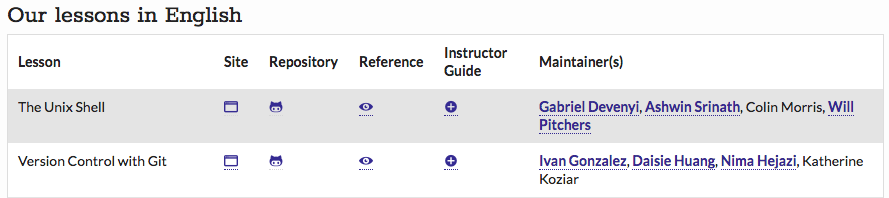
\includegraphics{../figures/talk/swc2.png}

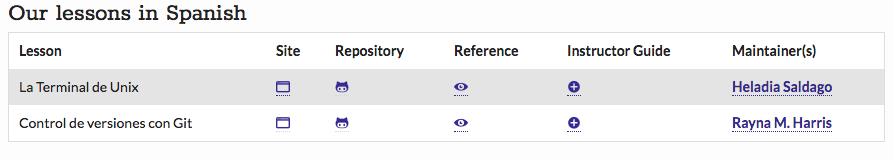
\includegraphics{../figures/talk/swc3.png} \footnote<.->{\url{https://software-carpentry.org/lessons/}}

\end{frame}

\begin{frame}{Mis 10 mejores deseos (en lugar de mis 10 mejores
consejos)}

\begin{itemize}[<+->]
\item
\item
  Recuerda: Vos podés hacer lo que quieras
\item
  Recuerda: Nadie es re buena al principio
\item
  Yo creo que la mejor manera de aprender es a ensenñar
\item
  Yo creo que todos aprenden más cuando la ciencia y la educación están
  abiertas
\end{itemize}

\end{frame}

\begin{frame}{Deseo 1: Usa \emph{R Markdown} para la reproducibilidad}

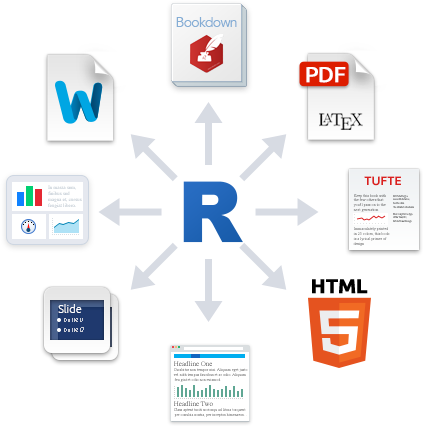
\includegraphics[width=0.50000\textwidth]{../figures/talk/Rmarkdown.png}
\footnote<.->{\url{https://rmarkdown.rstudio.com/authoring_quick_tour.html}}

\end{frame}

\begin{frame}{Deseo 2: Usa el control de versiones para la colaboración}

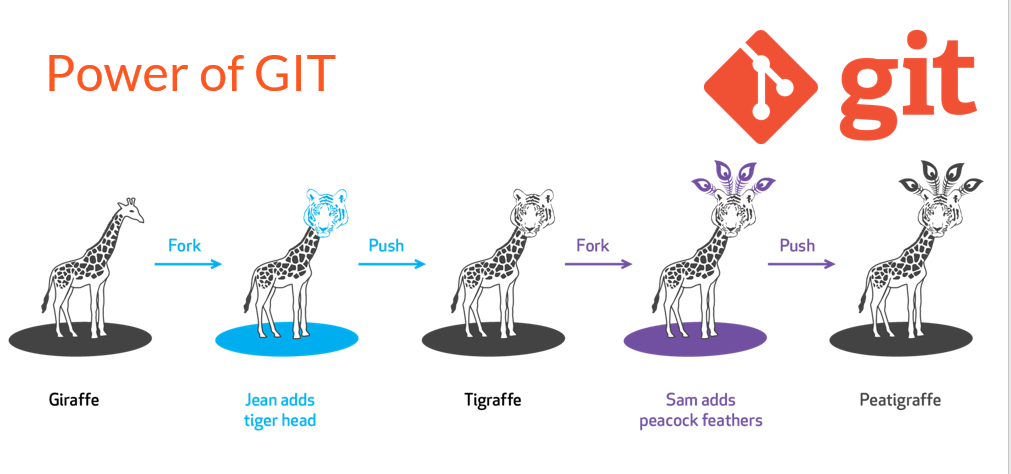
\includegraphics[width=0.75000\textwidth]{../figures/talk/git-graphic-01.png}
\footnote<.->{\url{http://technetnepal.net/blogs/shirishamaharjan/archive/2017/05/07/expand-horizons-change-attitudes-git-and-github-workshop.aspx}}

\end{frame}

\begin{frame}{Deseo 3: Documenta su flujo de trabajo}

Porque probablemente sea único y complejo

\includegraphics[width=0.75000\textwidth]{https://www.blogdelfotografo.com/wp-content/uploads/2016/05/mark-516279_1920.jpg}
{[}\^{}5{]} {[}\^{}5{]}:
\url{https://www.blogdelfotografo.com/workflow-flujo-trabajo-foto/}

\end{frame}

\begin{frame}{Por ejemplo, puede enumerar los comandos por orden de
operación}

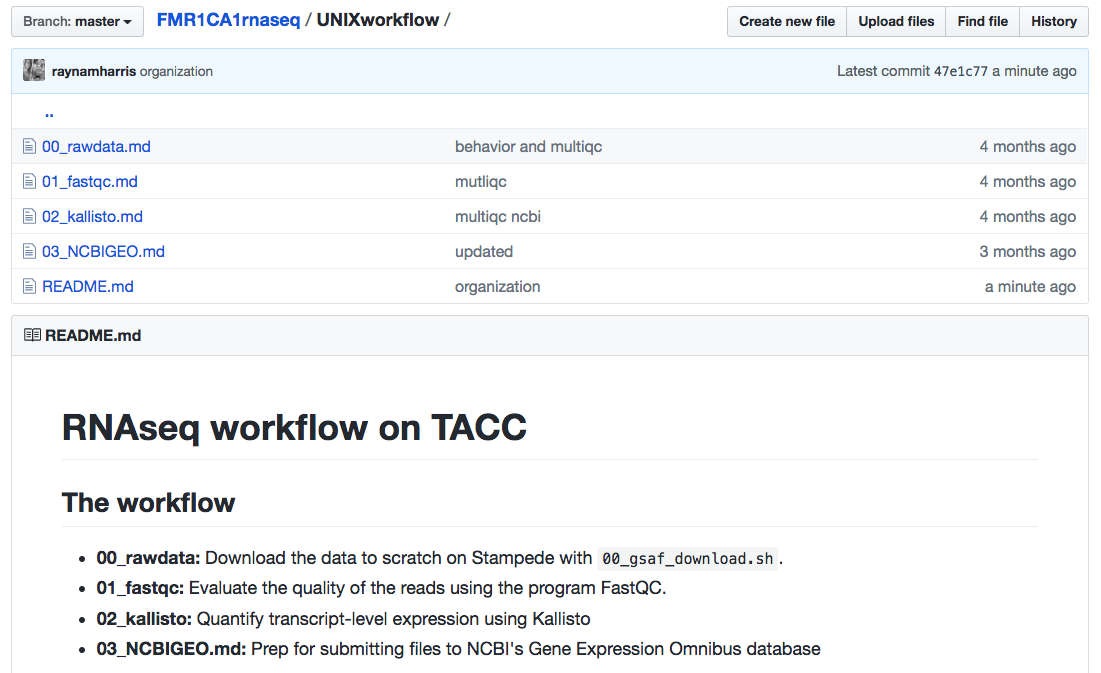
\includegraphics[width=0.75000\textwidth]{../figures/talk/unixworkflow.png}
\footnote<.->{\url{https://github.com/raynamharris/FMR1CA1rnaseq}}

\end{frame}

\begin{frame}{Pruebe múltiples estrategias de organización y haga lo que
funcione mejor para vos}

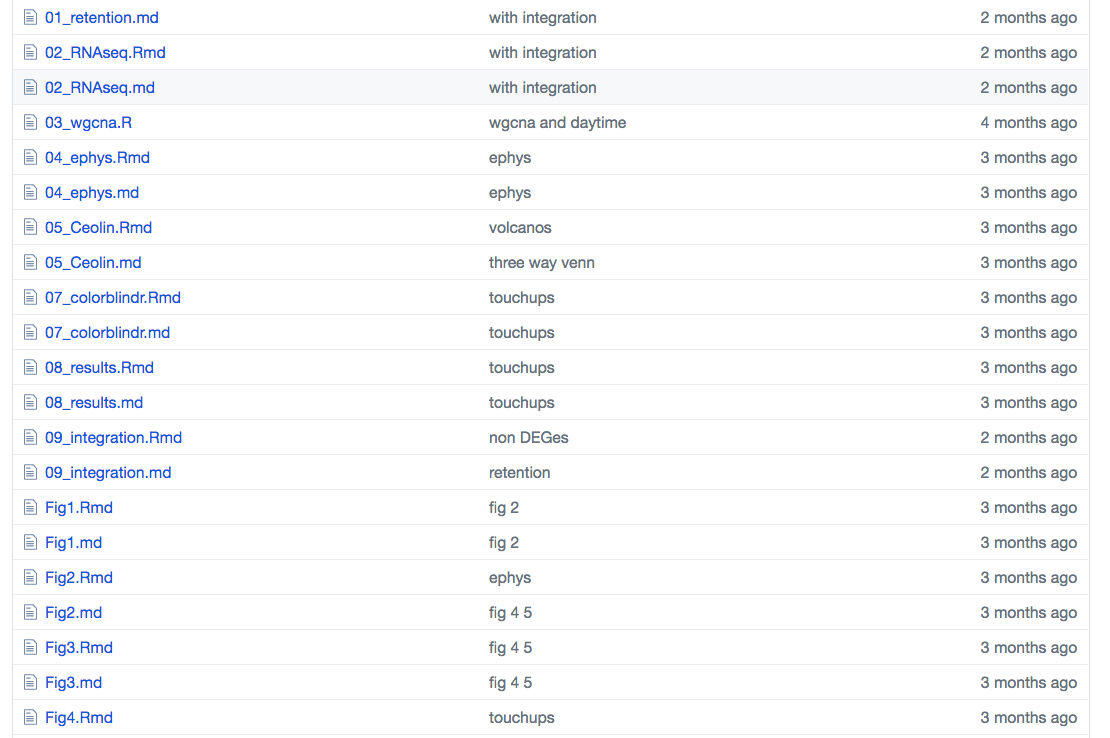
\includegraphics[width=0.75000\textwidth]{../figures/talk/Rworkflow.png}
\footnote<.->{\url{https://github.com/raynamharris/FMR1CA1rnaseq}}

\end{frame}

\begin{frame}{Deseo 4: Desarrolla tu propia paleta de colores}

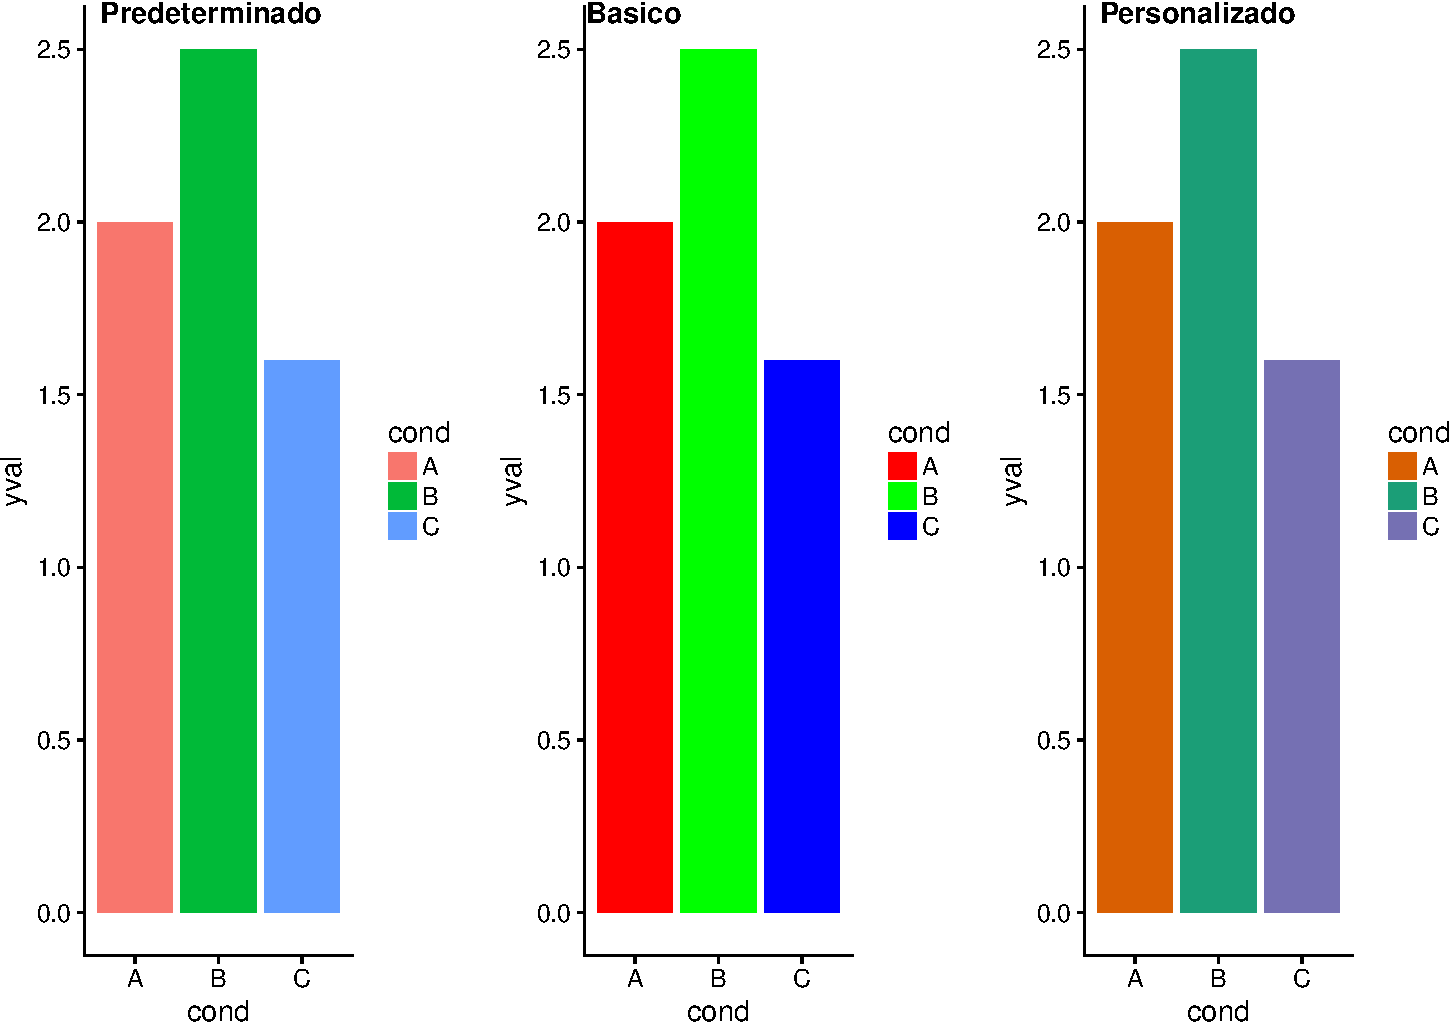
\includegraphics[width=250px]{../figures/talk/unnamed-chunk-1-1}

\begin{itemize}
\tightlist
\item
  I: predeterminado
\item
  II: values=c(``red'', ``green'', ``blue'')
\item
  III: values=c(``\#CC6666'', ``\#66CC99'', ``\#9999CC'')
\end{itemize}

\end{frame}

\begin{frame}{Deseo 4: Desarrolla tu propia paleta de colores}

Colorbrewer\footnote<.->{\url{http://colorbrewer2.org/}} te ayuda a
elegir colores amigables para el daltónico

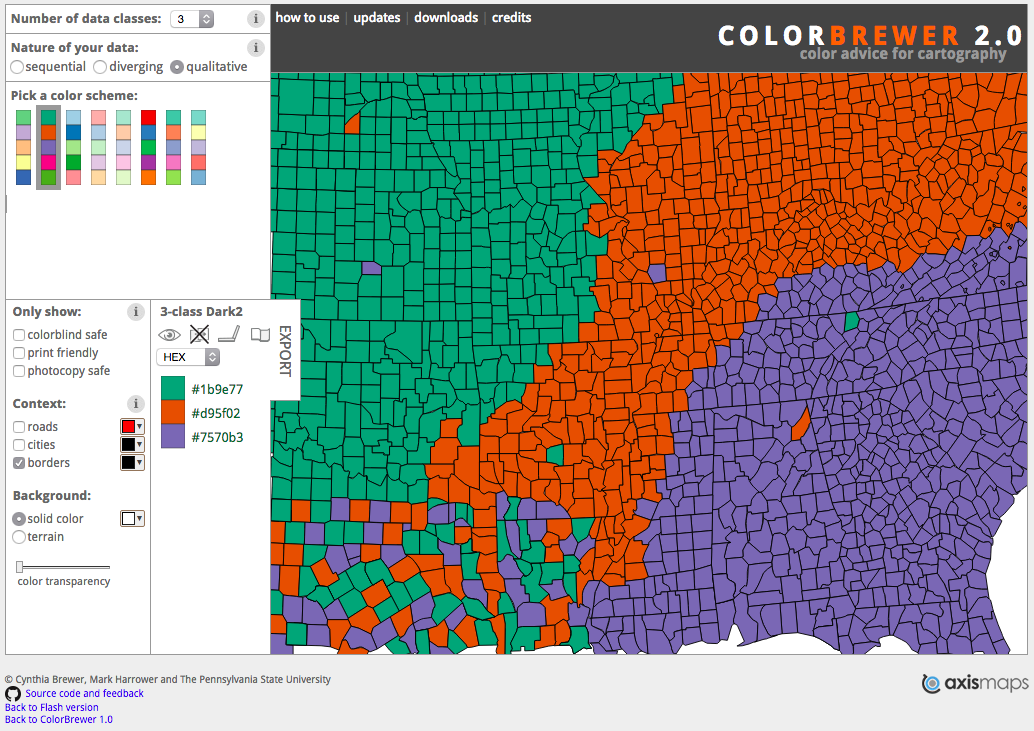
\includegraphics[width=0.75000\textwidth]{../figures/talk/colorbrewer.png}

\end{frame}

\begin{frame}{Deseo 5: Usa leyendas graficas}

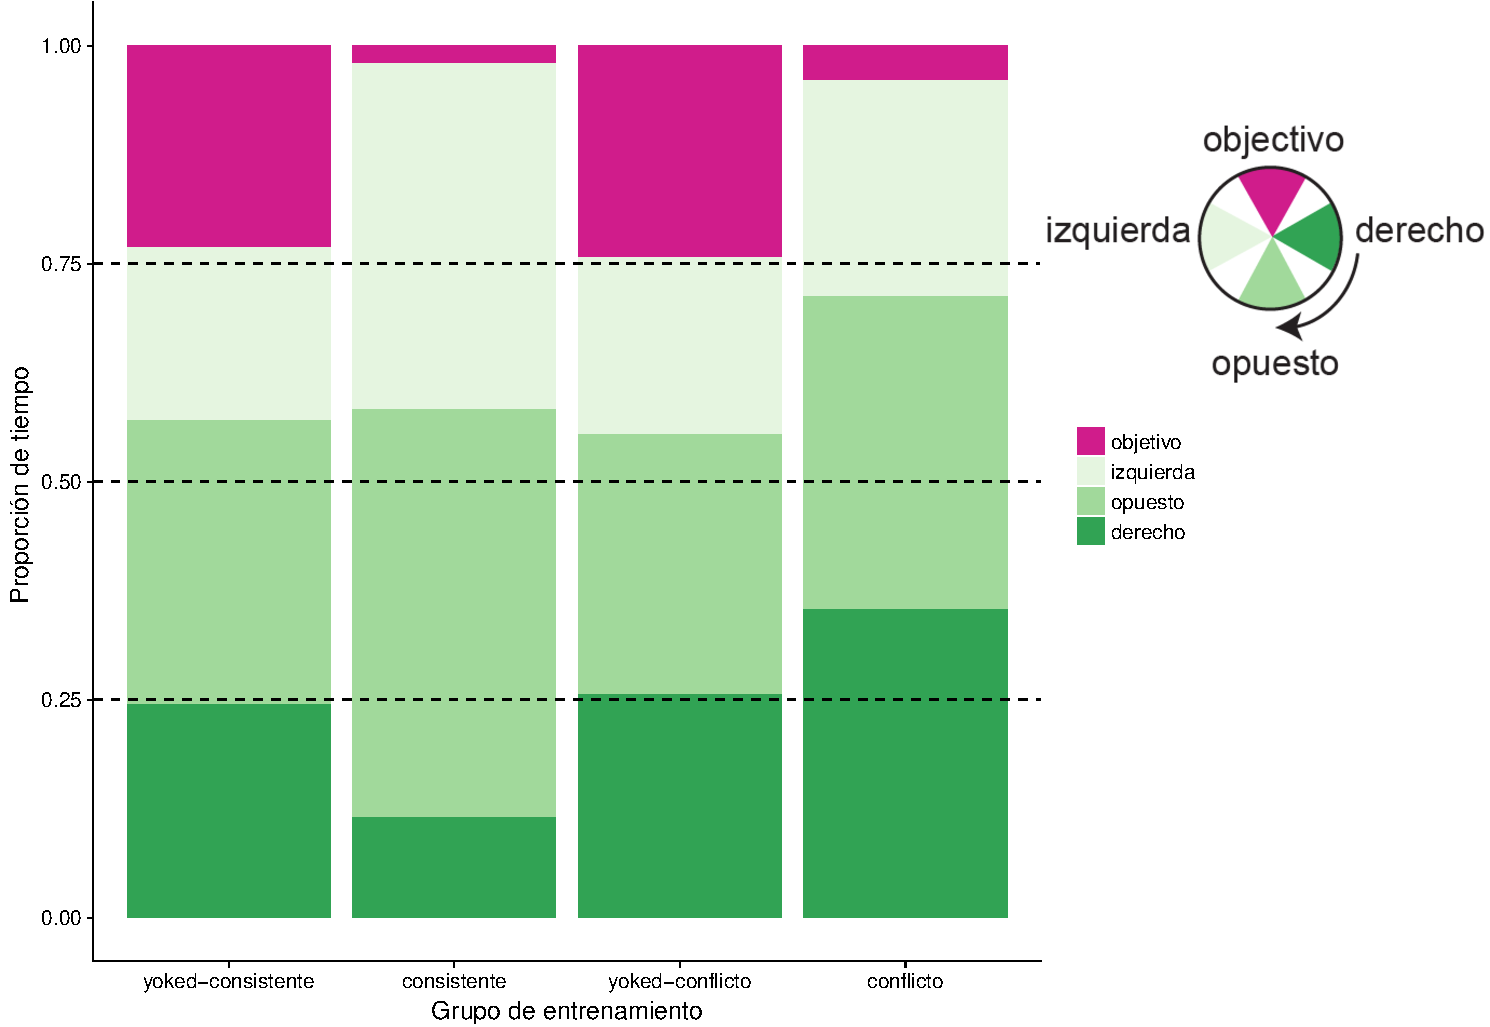
\includegraphics{../figures/talk/timespent-1.pdf}

\begin{itemize}[<+->]
\tightlist
\item
  ¿Qué significa ``objetivo'', ``izquierda'', ``opuesto'' y ``derecho''?
\item
  ¿Por qué el rosa ``objetivo''?
\item
  ¿Por qué hay líneas discontinuas?
\end{itemize}

\end{frame}

\begin{frame}{Deseo 5: Usa leyendas graficas}

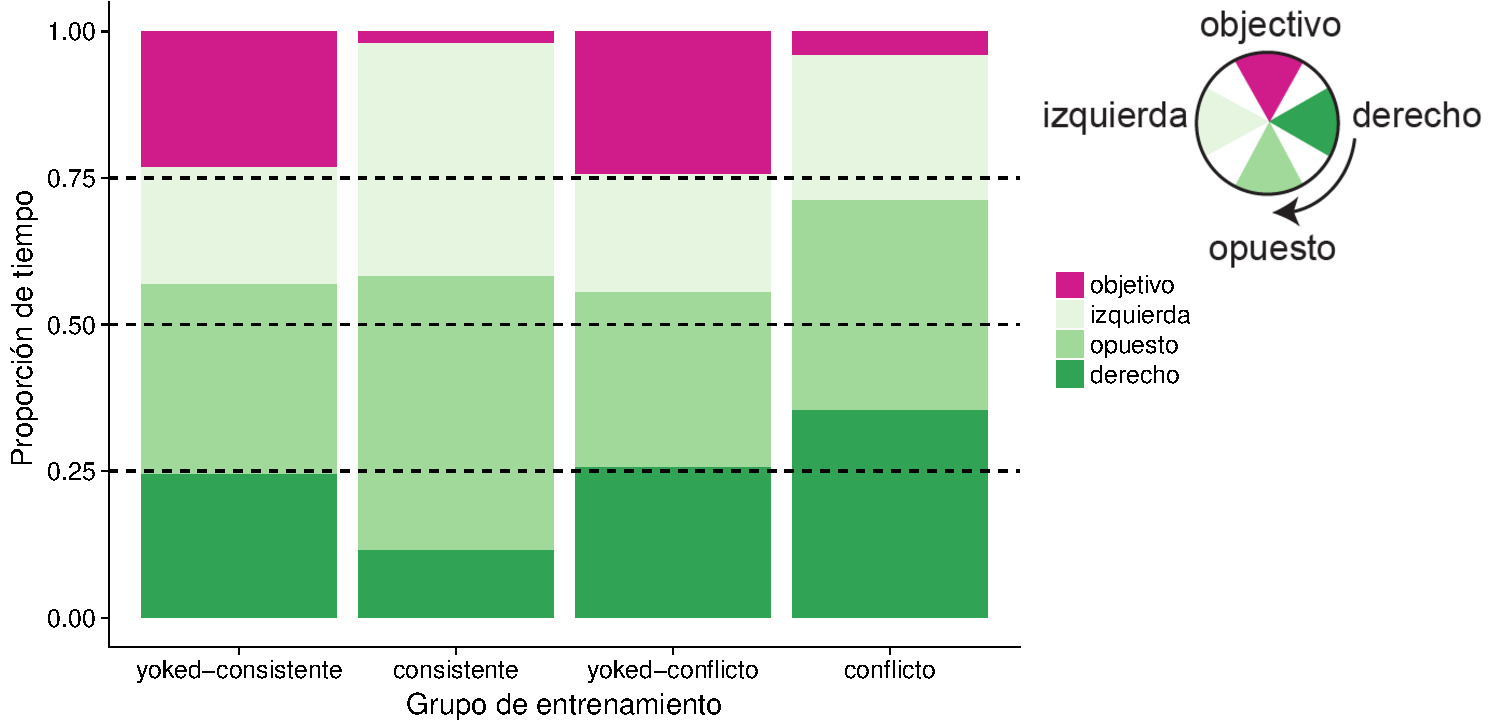
\includegraphics{../figures/talk/timespent2-1.pdf}

\begin{itemize}[<+->]
\tightlist
\item
  ``objetivo'', ``izquierda'', etc. son cuadrantes de una arena
\item
  Yo quería mostrar un uso desproporcionado del espacio
\item
  \textbf{cowplot}\footnote<.->{\textbf{cowplot}
    \url{https://cran.r-project.org/web/packages/cowplot/index.html}} es
  genial!
\end{itemize}

\end{frame}

\begin{frame}{En resumen}

\begin{itemize}
\tightlist
\item
  Deseo 1: Usa \emph{R Markdown} para la reproducibilidad
\item
  Deseo 2: Usa el control de versiones para la colaboración
\item
  Deseo 3: Documenta su flujo de trabajo
\item
  Deseo 4: Desarrolla tu propia paleta de colores
\item
  Deseo 5: Usa leyendas graficas
\end{itemize}

\end{frame}

\begin{frame}{Deseo 6: Me ayuda mejor las lecciones de Software
Carpentry}

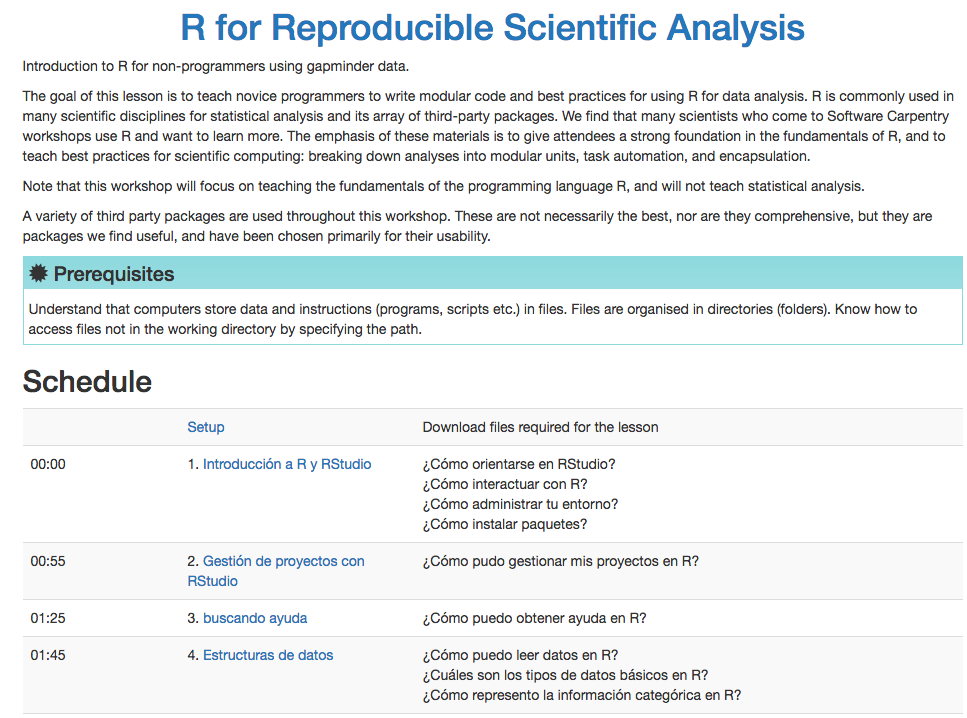
\includegraphics{../figures/talk/R-gapminder-es.png}

\end{frame}

\begin{frame}{Como puedes ayudar}

\begin{itemize}[<+->]
\tightlist
\item
  Leer y comentar o editar en GitHub
\item
  Particpar en el \textbf{Bug BBQ} el Abril 11 y 12
\item
  Organizar un taller o reunion para usarla
\item
  Haga videos de usted leyendo y codificando junto con la lección
\end{itemize}

\end{frame}

\begin{frame}{Deseo 7: Convertirse en una instructor certificada}

\begin{itemize}[<+->]
\tightlist
\item
  Aplicar aquí: \url{http://carpentries.github.io/instructor-training/}
\end{itemize}

\end{frame}

\begin{frame}{¡Gracias por su atención! ¡Mantengamonos en contacto!}

Twitter: @raynamharris Email:
\href{mailto:rayna.harris@gmail.com}{\nolinkurl{rayna.harris@gmail.com}}

\end{frame}

\end{document}
